\begin{acquis}
\begin{itemize}
\item BlaBla1
\item BlaBla2
\item BlaBla3
\item BlaBla4
\item BlaBla5
\item BlaBla6
\end{itemize}
\end{acquis}

\QCMautoevaluation{Pour chaque question, plusieurs réponses sont
  proposées.  Déterminer celles qui sont correctes.}

\begin{QCM}
  \begin{GroupeQCM}
    \begin{exercice}
      \begin{center} 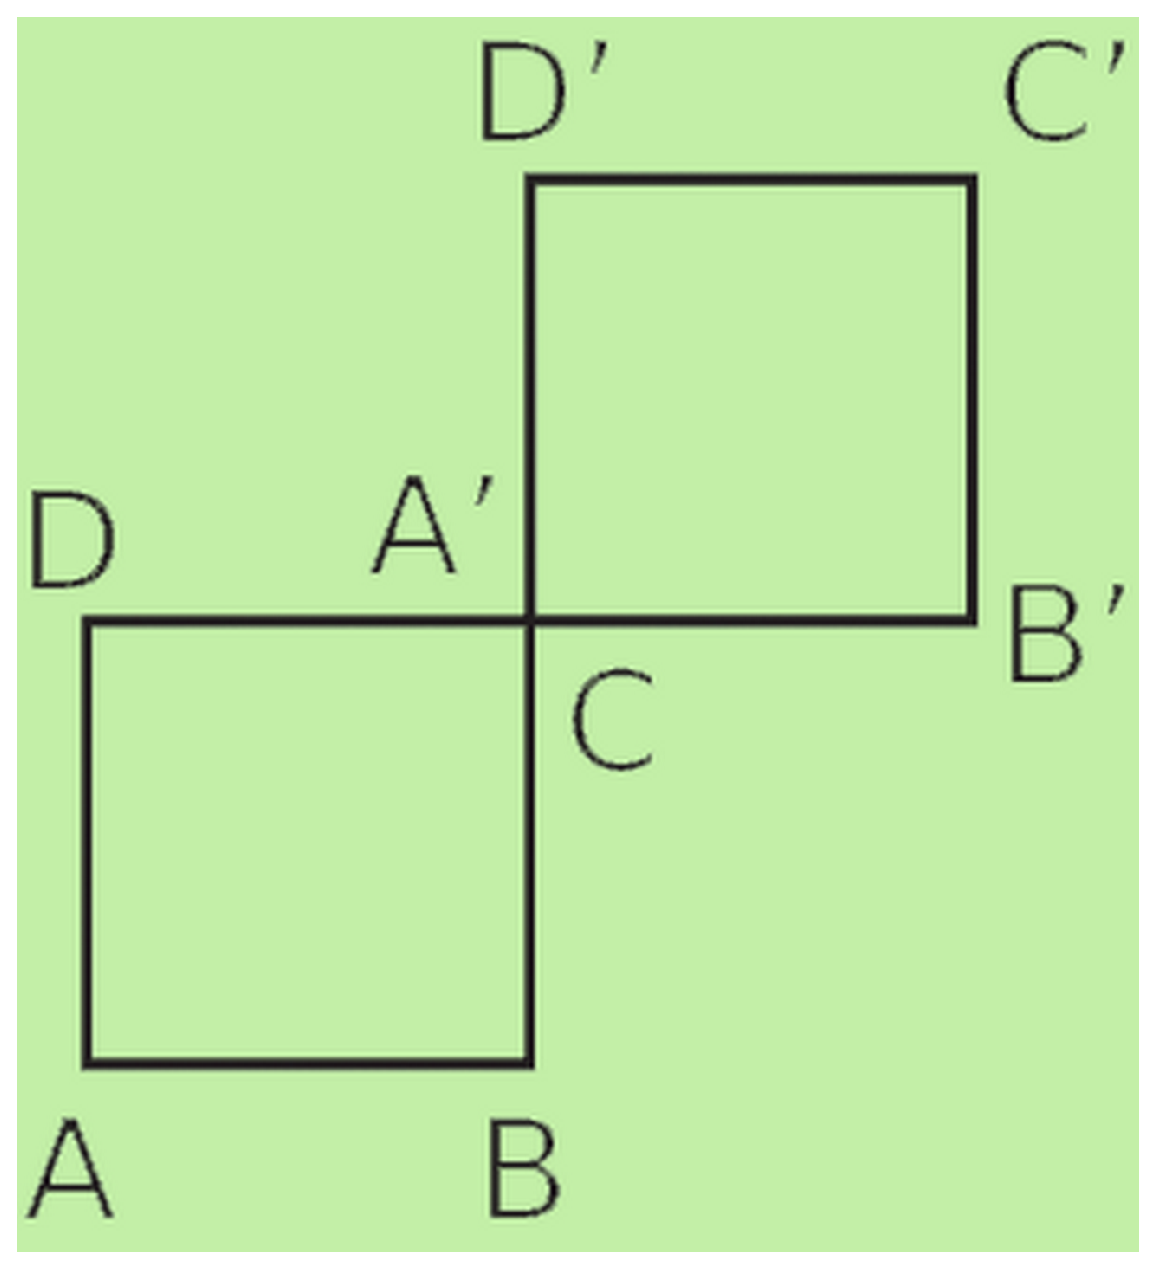
\includegraphics[width=2.6cm]{carreABCD_qcm} \end{center}
      \begin{center} Le carré $A'B'C'D'$ est l'image du carré $ABCD$ par la translation de vecteur \ldots \end{center}
      \begin{ChoixQCM}{4}
      \item $\overrightarrow{AB}$
      \item $\overrightarrow{AC}$
      \item $\overrightarrow{AD}$
      \item $\overrightarrow{BD}$
      \end{ChoixQCM}
\begin{corrige}
     \reponseQCM{a} % j'ai mis "a" partout
   \end{corrige}
    \end{exercice}
    
    
    \begin{exercice}
      \begin{center} 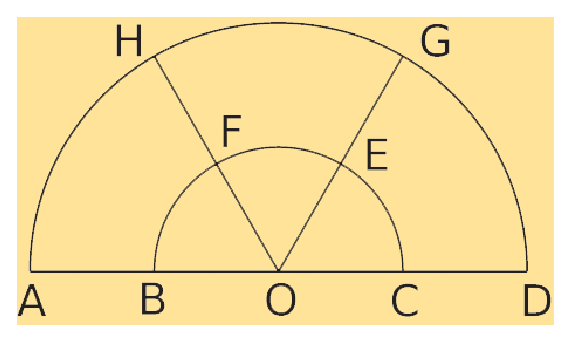
\includegraphics[width=4.2cm]{equerre_rotation_qcm} \end{center}
      \begin{center} $E$ est l'image de $F$ par la rotation de centre $O$ et d'angle \ldots \end{center}
      \begin{ChoixQCM}{4}
      \item $+ 30^\circ$
      \item $- 30^\circ$
      \item $+ 60^\circ$
      \item $- 60^\circ$
      \end{ChoixQCM}
\begin{corrige}
     \reponseQCM{a}
   \end{corrige}
    \end{exercice}
    
    
    \begin{exercice}
      Sur l'image ci-dessus, l'image de $D$ par une rotation de centre $O$ et d'angle $120^\circ$ est \ldots
      \begin{ChoixQCM}{4}
      \item $A$
      \item $H$
      \item $G$
      \item $O$
      \end{ChoixQCM}
\begin{corrige}
     \reponseQCM{a}
   \end{corrige}
    \end{exercice}


\end{GroupeQCM}
\end{QCM}

  